\documentclass{article}\usepackage[]{graphicx}\usepackage[]{color}
%% maxwidth is the original width if it is less than linewidth
%% otherwise use linewidth (to make sure the graphics do not exceed the margin)
\makeatletter
\def\maxwidth{ %
  \ifdim\Gin@nat@width>\linewidth
    \linewidth
  \else
    \Gin@nat@width
  \fi
}
\makeatother

\definecolor{fgcolor}{rgb}{0.345, 0.345, 0.345}
\newcommand{\hlnum}[1]{\textcolor[rgb]{0.686,0.059,0.569}{#1}}%
\newcommand{\hlstr}[1]{\textcolor[rgb]{0.192,0.494,0.8}{#1}}%
\newcommand{\hlcom}[1]{\textcolor[rgb]{0.678,0.584,0.686}{\textit{#1}}}%
\newcommand{\hlopt}[1]{\textcolor[rgb]{0,0,0}{#1}}%
\newcommand{\hlstd}[1]{\textcolor[rgb]{0.345,0.345,0.345}{#1}}%
\newcommand{\hlkwa}[1]{\textcolor[rgb]{0.161,0.373,0.58}{\textbf{#1}}}%
\newcommand{\hlkwb}[1]{\textcolor[rgb]{0.69,0.353,0.396}{#1}}%
\newcommand{\hlkwc}[1]{\textcolor[rgb]{0.333,0.667,0.333}{#1}}%
\newcommand{\hlkwd}[1]{\textcolor[rgb]{0.737,0.353,0.396}{\textbf{#1}}}%

\usepackage{framed}
\makeatletter
\newenvironment{kframe}{%
 \def\at@end@of@kframe{}%
 \ifinner\ifhmode%
  \def\at@end@of@kframe{\end{minipage}}%
  \begin{minipage}{\columnwidth}%
 \fi\fi%
 \def\FrameCommand##1{\hskip\@totalleftmargin \hskip-\fboxsep
 \colorbox{shadecolor}{##1}\hskip-\fboxsep
     % There is no \\@totalrightmargin, so:
     \hskip-\linewidth \hskip-\@totalleftmargin \hskip\columnwidth}%
 \MakeFramed {\advance\hsize-\width
   \@totalleftmargin\z@ \linewidth\hsize
   \@setminipage}}%
 {\par\unskip\endMakeFramed%
 \at@end@of@kframe}
\makeatother

\definecolor{shadecolor}{rgb}{.97, .97, .97}
\definecolor{messagecolor}{rgb}{0, 0, 0}
\definecolor{warningcolor}{rgb}{1, 0, 1}
\definecolor{errorcolor}{rgb}{1, 0, 0}
\newenvironment{knitrout}{}{} % an empty environment to be redefined in TeX

\usepackage{alltt}

\usepackage{fancyhdr} % Required for custom headers
\usepackage{lastpage} % Required to determine the last page for the footer
\usepackage{extramarks} % Required for headers and footers
\usepackage{graphicx} % Required to insert images
\usepackage{hyperref}
\usepackage{amsmath} %for binomial pdf
\usepackage{parskip} % so that there's space bw paragraphs
\usepackage{float}
\usepackage{amsfonts}
\usepackage{hanging}
\usepackage{undertilde}
\usepackage{amssymb}
\usepackage{graphicx} %include images


% Margins
\topmargin=-0.45in
\evensidemargin=0in
\oddsidemargin=0in
\textwidth=6.5in
\textheight=9.0in
\headsep=0.25in 

\linespread{1.1} % Line spacing

% Set up the header and footer
\pagestyle{fancy}
\lhead{STAT 532: Bayes} % Top left header
\chead{HW 7} % Top center header
\rhead{Andrea Mack} % Top right header
\lfoot{11/18/2016} % Bottom left footer
\cfoot{} % Bottom center footer
\rfoot{Page\ \thepage\ of\ \pageref{LastPage}} % Bottom right footer
\renewcommand\headrulewidth{0.4pt} % Size of the header rule
\renewcommand\footrulewidth{0.4pt} % Size of the footer rule

\setlength\parindent{0pt} % Removes all indentation from paragraphs
\setlength\parskip{0.5cm}
\restylefloat{table}

%----------------------------------------------------------------------------------------
%	DOCUMENT STRUCTURE COMMANDS
%	Skip this unless you know what you're doing
%----------------------------------------------------------------------------------------

% Header and footer for when a page split occurs within a problem environment
\newcommand{\enterProblemHeader}[1]{
\nobreak\extramarks{#1}{#1 continued on next page\ldots}\nobreak
\nobreak\extramarks{#1 (continued)}{#1 continued on next page\ldots}\nobreak
}

% Header and footer for when a page split occurs between problem environments
\newcommand{\exitProblemHeader}[1]{
\nobreak\extramarks{#1 (continued)}{#1 continued on next page\ldots}\nobreak
\nobreak\extramarks{#1}{}\nobreak
}


%----------------------------------------------------------------------------------------%
\IfFileExists{upquote.sty}{\usepackage{upquote}}{}
\begin{document}


\begin{enumerate}
\item%1 
{\it (10 points) Under Zellner's g-prior $\Sigma_{o} = \sigma^2(X^{T}X)^{-1}$, with $\utilde{\beta_{o}} = \utilde{0}$, state your prior for $\sigma^{2}$ and derive the marginal distribution p($\sigma{2} | \utilde{y},X$).}
$\gamma = \frac{1}{\sigma^2} \sim$ GAM($\frac{\nu_{o} + n}{2},(\nu_{o}\sigma_{o}^{2} + SSR_{g})/2$)

$\gamma = \frac{1}{\sigma^{2}} \sim$ GAM($\frac{\nu_{o}}{2},\nu_{o}\sigma_{o}^{2}/2$)

p($\gamma | \utilde{y},\utilde{x}$) \propto $p(\gamma)p(\utilde{y} | \utilde{X},\gamma)$

Generally we think p($\gamma | \utilde{y},\utilde{x}, \beta$) \propto $p(\utilde{y} | \utilde{X},\gamma, \beta)p(\gamma | \beta)p(\beta)$,

but for the same reason as the previous homework, {\it which I still don't understand}, we can simplify and remove the $\beta$ terms.

We have:
p($\frac{1}{\sigma^2} | \utilde{y},\utilde{x}$) \propto $p(\frac{1}{\sigma^2})p(\utilde{y} | \utilde{X},\frac{1}{\sigma^2})$

\propto $(\frac{1}{\sigma^2})^{\nu_{o}/2 - 1}exp(-\frac{1}{\sigma^2}[\nu_{o}\sigma^2_{o}/2) \times (\frac{1}{\sigma^2})^{n/2}exp(-\frac{1}{2\sigma^2}(\utilde{Y} - \utilde{x}\beta)^{T}(\utilde{Y} - \utilde{x}\beta))$

\propto $\frac{1}{\sigma^2}^{(\nu_{o} + n)/2} \times exp(-\frac{1}{2\sigma^{2}}[\nu_{o}\sigma^2_{o} + (\utilde{Y} - \utilde{X}\beta)^{T}(\utilde{Y} - \utilde{X}\beta)^{T}])$

\propto $\frac{1}{\sigma^2}^{(\nu_{o} + n)/2} \times exp(-\frac{1}{2\sigma^{2}}[\nu_{o}\simga^2_{o} + SSR])$

\item {\it (10 points) Describe the process for choosing priors in Bayesian hypothesis testing with Bayes
Factors.}

\item {\it Download the King County housing dataset from D2L. You have free rein to use this question
to apply some of the ideas we have learned in class. The goal is to create a predictive model
that best captures the housing dynamics in King County. Note, there is a dataset called
predictHouse, that contains all of the covariates, but will require a predicted price. This will
be part of the homework submission and all of the entries will be compared. Note you will only
be asked to provide a point estimate, but I could as for a posterior predictive distribution for
each home.}

\begin{enumerate}
\item {\it (10 points) What factors in the dataset to you anticipate being useful predictors of housing
price?}

Taken from Windermere Real Estate's website, below is a picture of King County Washington.

\begin{center}
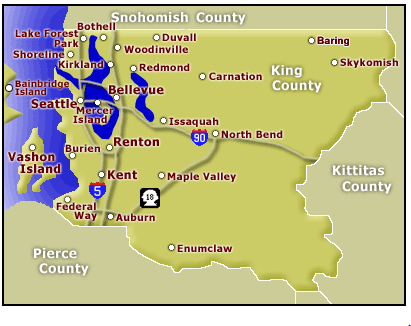
\includegraphics[scale = 0.75]{king_county}
\end{center}


\begin{knitrout}
\definecolor{shadecolor}{rgb}{0.969, 0.969, 0.969}\color{fgcolor}
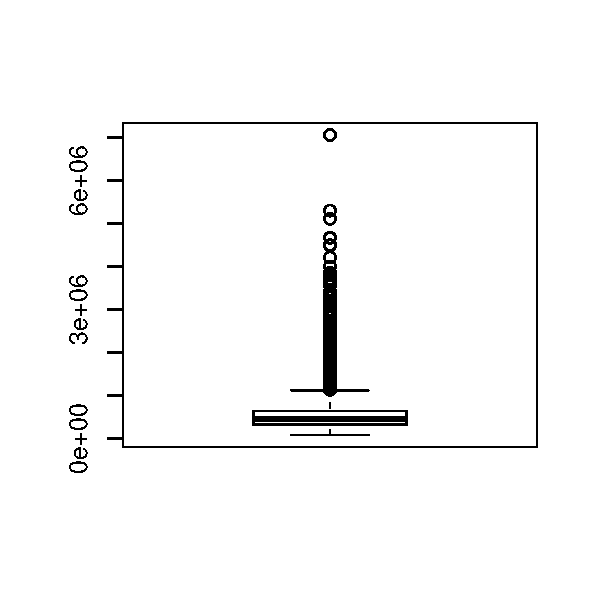
\includegraphics[width=\maxwidth]{figure/prob3a-1} 

\end{knitrout}

\begin{knitrout}
\definecolor{shadecolor}{rgb}{0.969, 0.969, 0.969}\color{fgcolor}\begin{kframe}
\begin{verbatim}
## as.geodata: 398 replicated data locations found. 
##  Consider using jitterDupCoords() for jittering replicated locations. 
## WARNING: there are data at coincident or very closed locations, some of the geoR's functions may not work.
##  Use function dup.coords() to locate duplicated coordinates.
##  Consider using jitterDupCoords() for jittering replicated locations
## [1] 379
\end{verbatim}
\end{kframe}
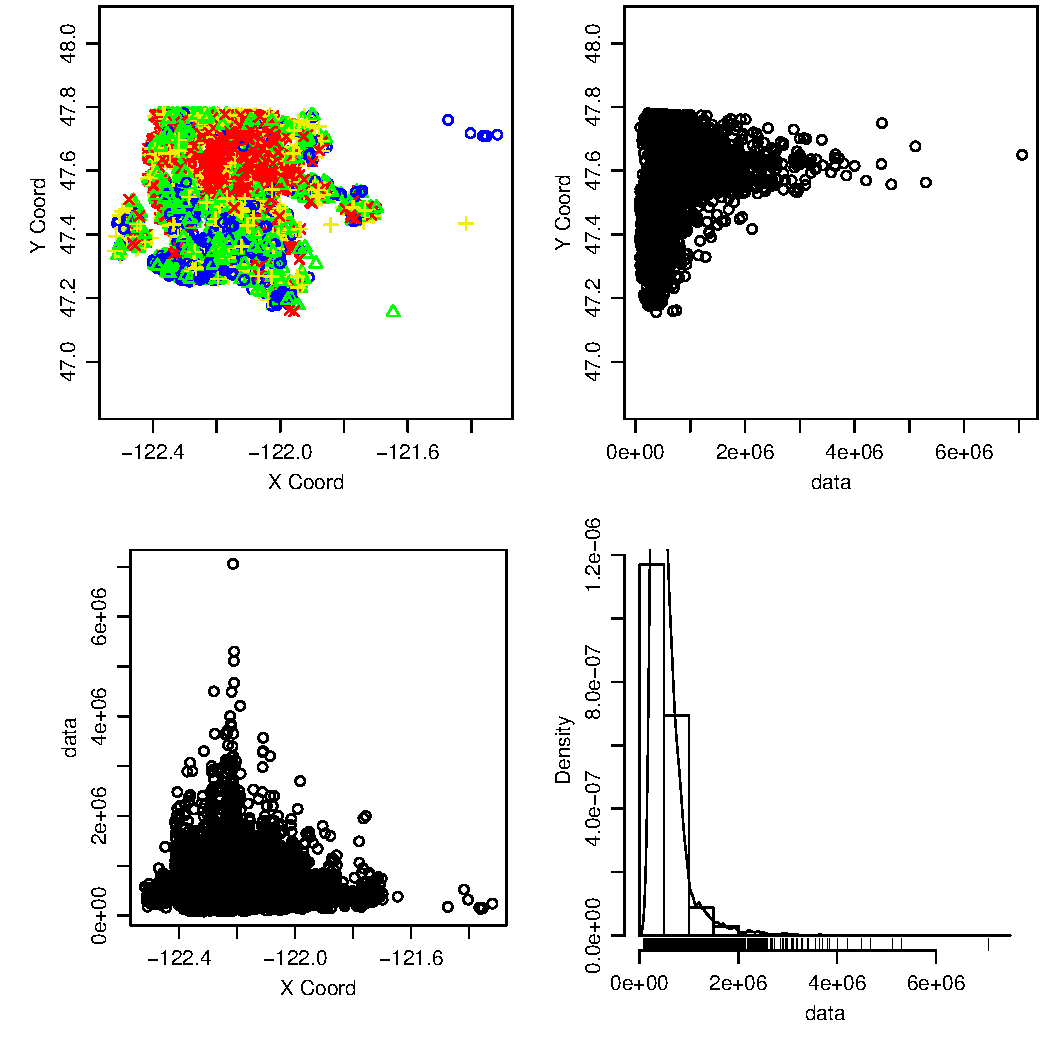
\includegraphics[width=\maxwidth]{figure/prob3ax-1} 

\end{knitrout}

The geo plot visualizes the area considered. If location coordinates did not affect price, the north east and south west plots would show random scatter. Prices at certain location coordinates are higher than others. There are also a few houses located farther from others. Perhaps zipcode will serve as a good enough proxy for location coordinates. A SLR model was fit to model price as a function of zipcode. Due to the increasing variation and the large right skew in the residuals, price was logged. Doing so made the constant variance and normality assumptions more reasonable, but not perfect. 

\begin{knitrout}
\definecolor{shadecolor}{rgb}{0.969, 0.969, 0.969}\color{fgcolor}
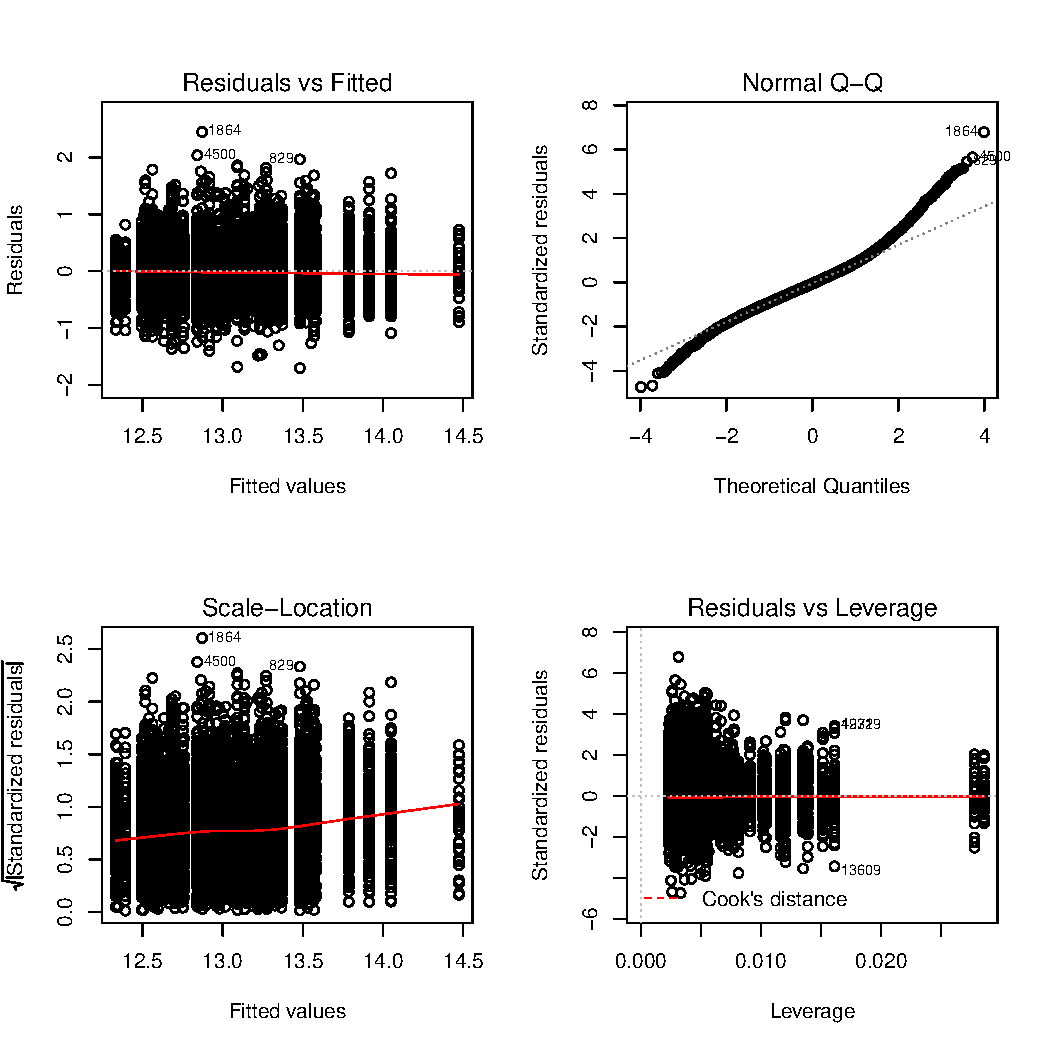
\includegraphics[width=\maxwidth]{figure/m1-1} 

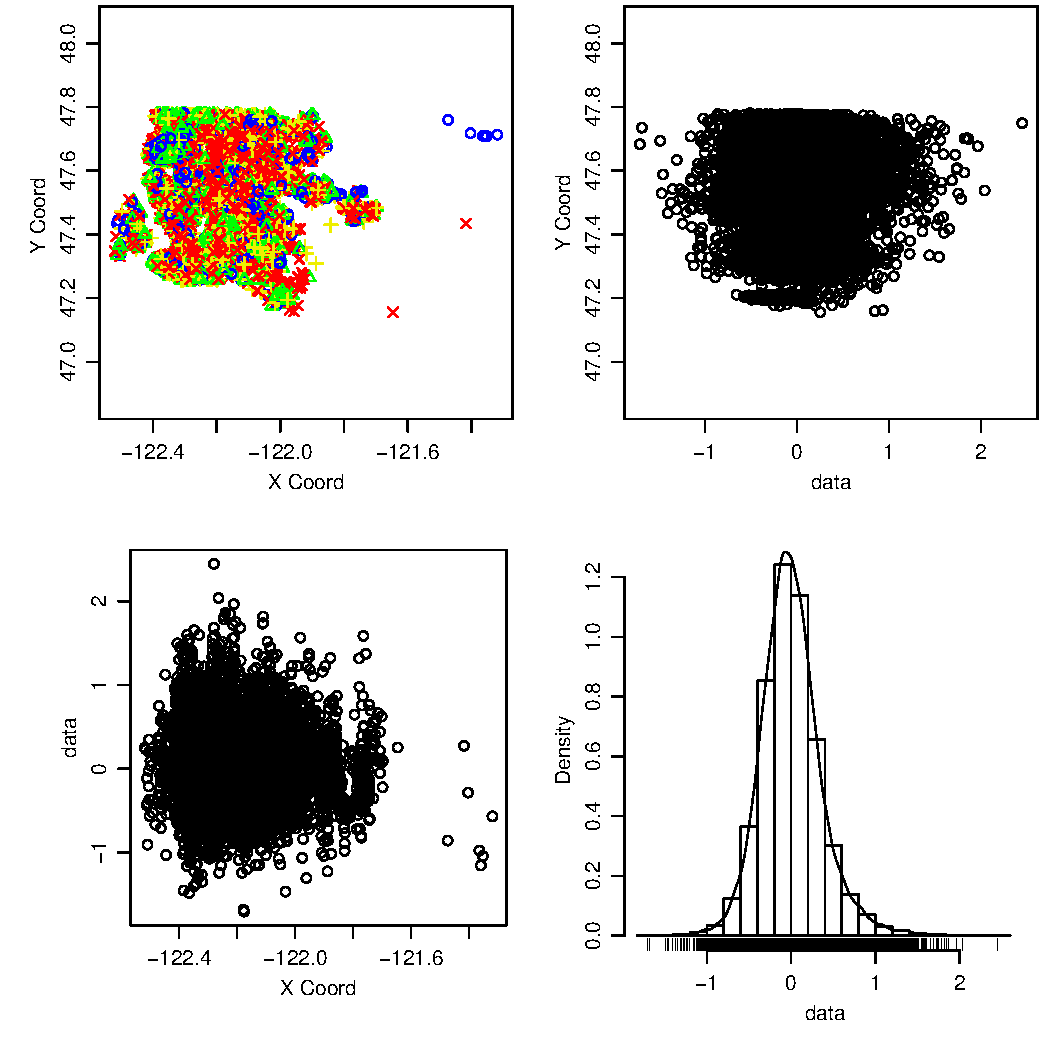
\includegraphics[width=\maxwidth]{figure/m1-2} 

\end{knitrout}

The off diagonal plots show random scatter, so relationships between price and location coordinates may be accounted for by including zipcode in the final model.

{\bf Note: zipcode is categorical!}

With 23 possible covariates, I chose six continuous or reasonably approximately continuous variables to see how correlated they were.



\begin{knitrout}
\definecolor{shadecolor}{rgb}{0.969, 0.969, 0.969}\color{fgcolor}
\includegraphics[width=\maxwidth]{figure/pairs-1} 

\includegraphics[width=\maxwidth]{figure/pairs-2} 

\end{knitrout}

One of the levels forth year renovated is ``0", which is most likely a miss code. Zeros for the renovated variable imply not renovated. Only a small proportion (4.2897746\%) of the houses were renovated.

\begin{knitrout}
\definecolor{shadecolor}{rgb}{0.969, 0.969, 0.969}\color{fgcolor}\begin{kframe}
\begin{verbatim}
##  [1] 1 1 1 1 1 1 1 1 1 1 1 1 1 1 1 1 1 1 1 1 1 1 1 1 1 1 1 1 1 1 1 1 1 1 1
\end{verbatim}
\end{kframe}
\end{knitrout}

Based on the EDA, I think zipcode will be important to counteract location coordinates, though a model with variation relative to spatical coordinates would be most accurate. After accounting for zipcode, I do not think location coordinates will affect variation in prices.

Many of the continuous variables are on much different scales and the effects of variables on a small scale may be masked by effects of variables on a large scale, therefore, all continuous variables were scaled and centered. Bathrooms have fractional levels, and so bathrooms was also considered as continuous, scaled and centered.

Continuous (or the like) Variables:

Based on the pairwise correlation plots, I believe either square footage or the average square footage of the 15 nearest houses will be important. The number of bathrooms and number of bedrooms also may be important with correlations to price of 0.52 and 0.3 respectively, as the two are highly correlated to each other, the effect of bathrooms may mask the effect of bedrooms.

\begin{knitrout}
\definecolor{shadecolor}{rgb}{0.969, 0.969, 0.969}\color{fgcolor}
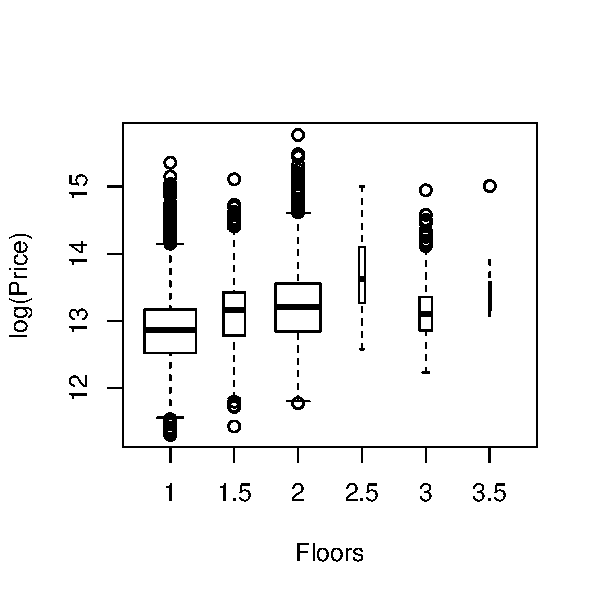
\includegraphics[width=\maxwidth]{figure/discrete-1} 

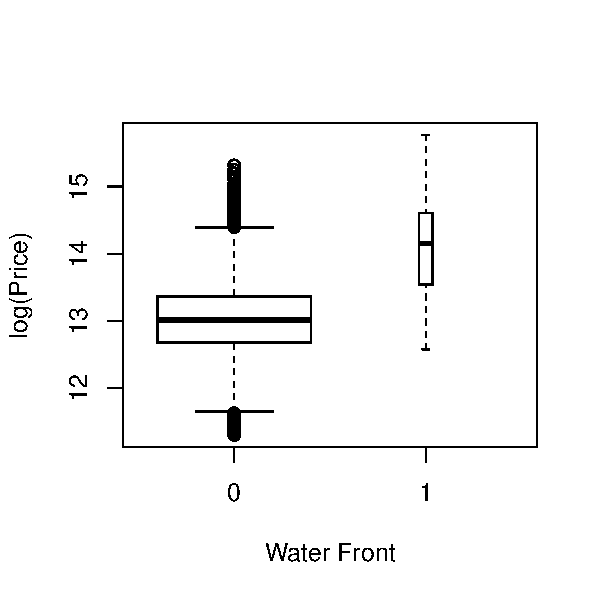
\includegraphics[width=\maxwidth]{figure/discrete-2} 

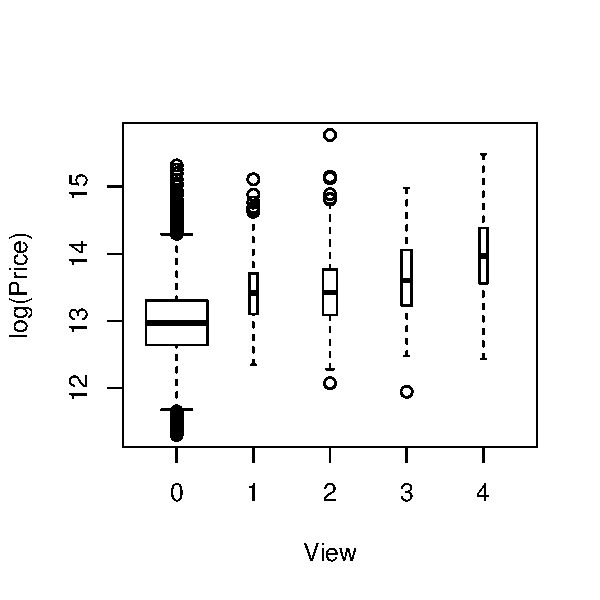
\includegraphics[width=\maxwidth]{figure/discrete-3} 

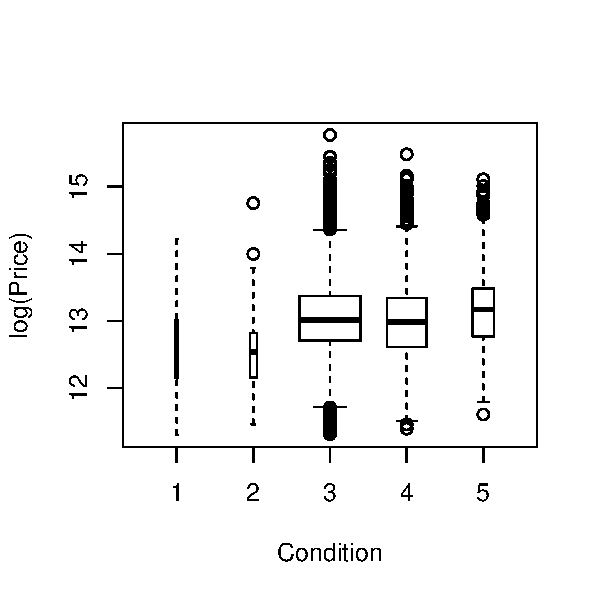
\includegraphics[width=\maxwidth]{figure/discrete-4} 

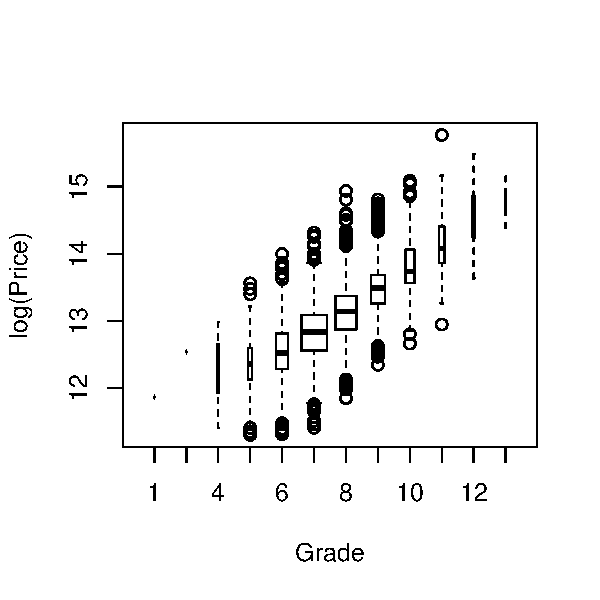
\includegraphics[width=\maxwidth]{figure/discrete-5} 

\end{knitrout}


Waterfront, view, and grade all look like they may affect price, with view and grade on an exponential level. 

\begin{knitrout}
\definecolor{shadecolor}{rgb}{0.969, 0.969, 0.969}\color{fgcolor}\begin{kframe}


{\ttfamily\noindent\itshape\color{messagecolor}{\#\# Loading required package: stringr}}\end{kframe}
\end{knitrout}

\begin{knitrout}
\definecolor{shadecolor}{rgb}{0.969, 0.969, 0.969}\color{fgcolor}
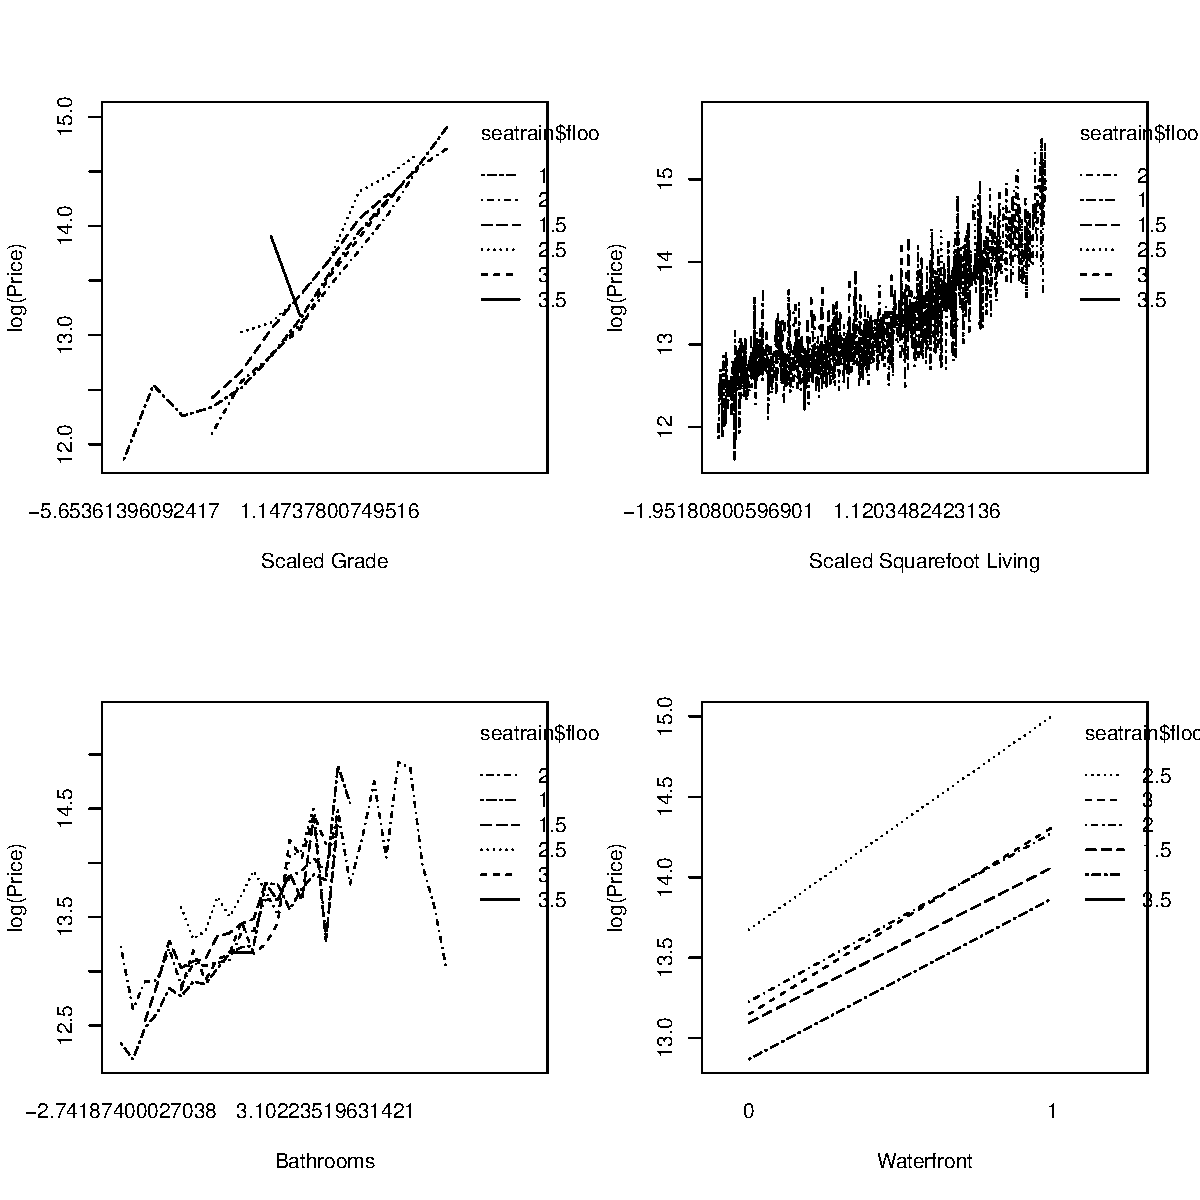
\includegraphics[width=\maxwidth]{figure/interact-1} 

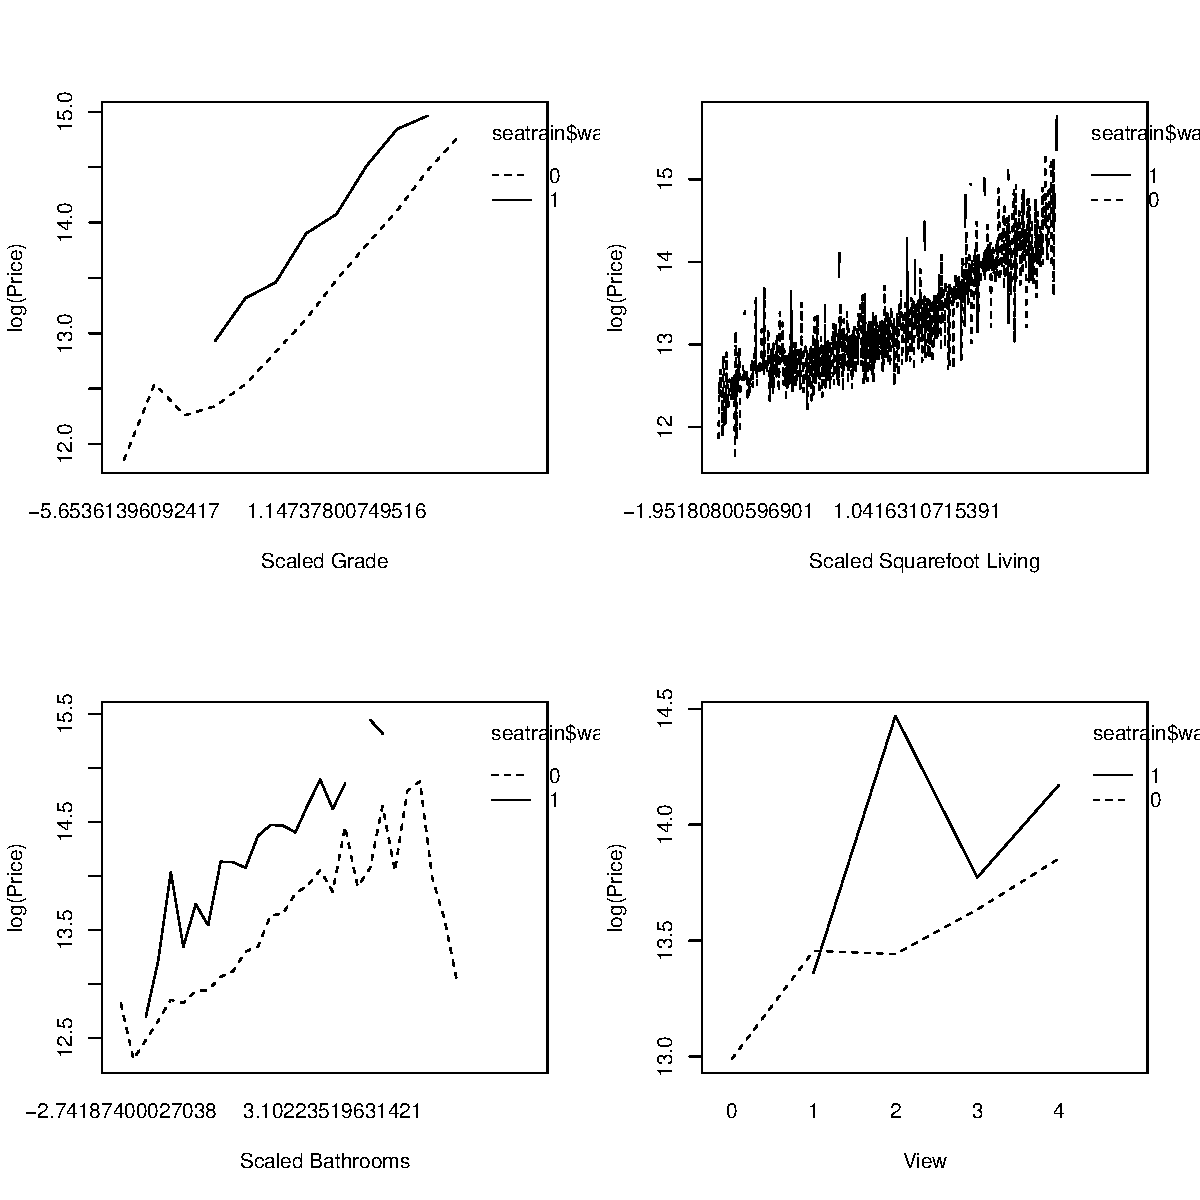
\includegraphics[width=\maxwidth]{figure/interact-2} 

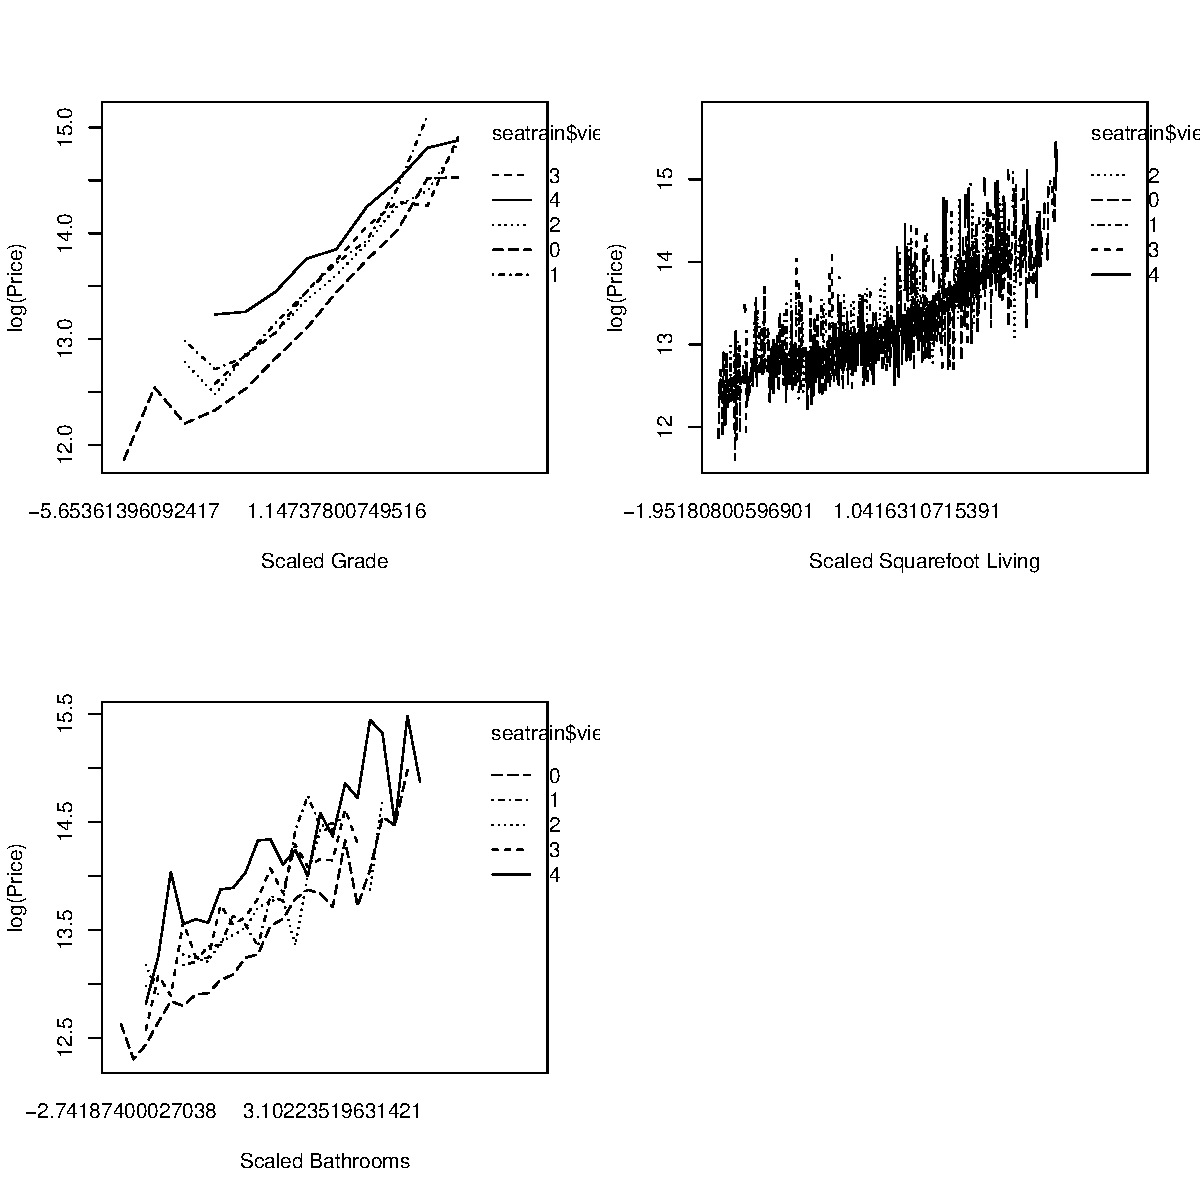
\includegraphics[width=\maxwidth]{figure/interact-3} 

\end{knitrout}



\item%3b

{\it (10 points) What challenges did you face in understanding or processing the data?}

EDA took a long time, so it took a lot to understand the variables and get to the point where I could try out model selection in terms of Bayes.
\end{enumerate}

\section*{R Code}
\begin{enumerate}
\setcounter{enumi}{3}
{\tiny
}
\end{enumerate}

\end{document}
